\documentclass[LaTeX2e,10pt,aspectratio=169]{beamer}
\setbeamertemplate{navigation symbols}{}
\usefonttheme[onlymath]{serif}

\usepackage{tikz}
\newcommand\w{0.12}

\usetikzlibrary{fit,positioning}
\tikzstyle{every picture}+=[remember picture]

\begin{document}

\bgroup
\setbeamercolor{background canvas}{bg=white}
\begin{frame}[plain]{}
	\begin{tikzpicture}[
    node distance = 7mm and -3mm,
every node/.style = {draw=black, rounded corners, fill=gray!30, 
                     minimum width=2cm, minimum height=0.5cm,
                     align=center}
                        ]
\node [label=$\tilde{x}$](scarceSinogram) {\includegraphics[width=\w\textwidth]{sophia_sin_example.png}};

\node [label=$G(\tilde{x})$](inpainted)  [right=5mm of scarceSinogram.east] {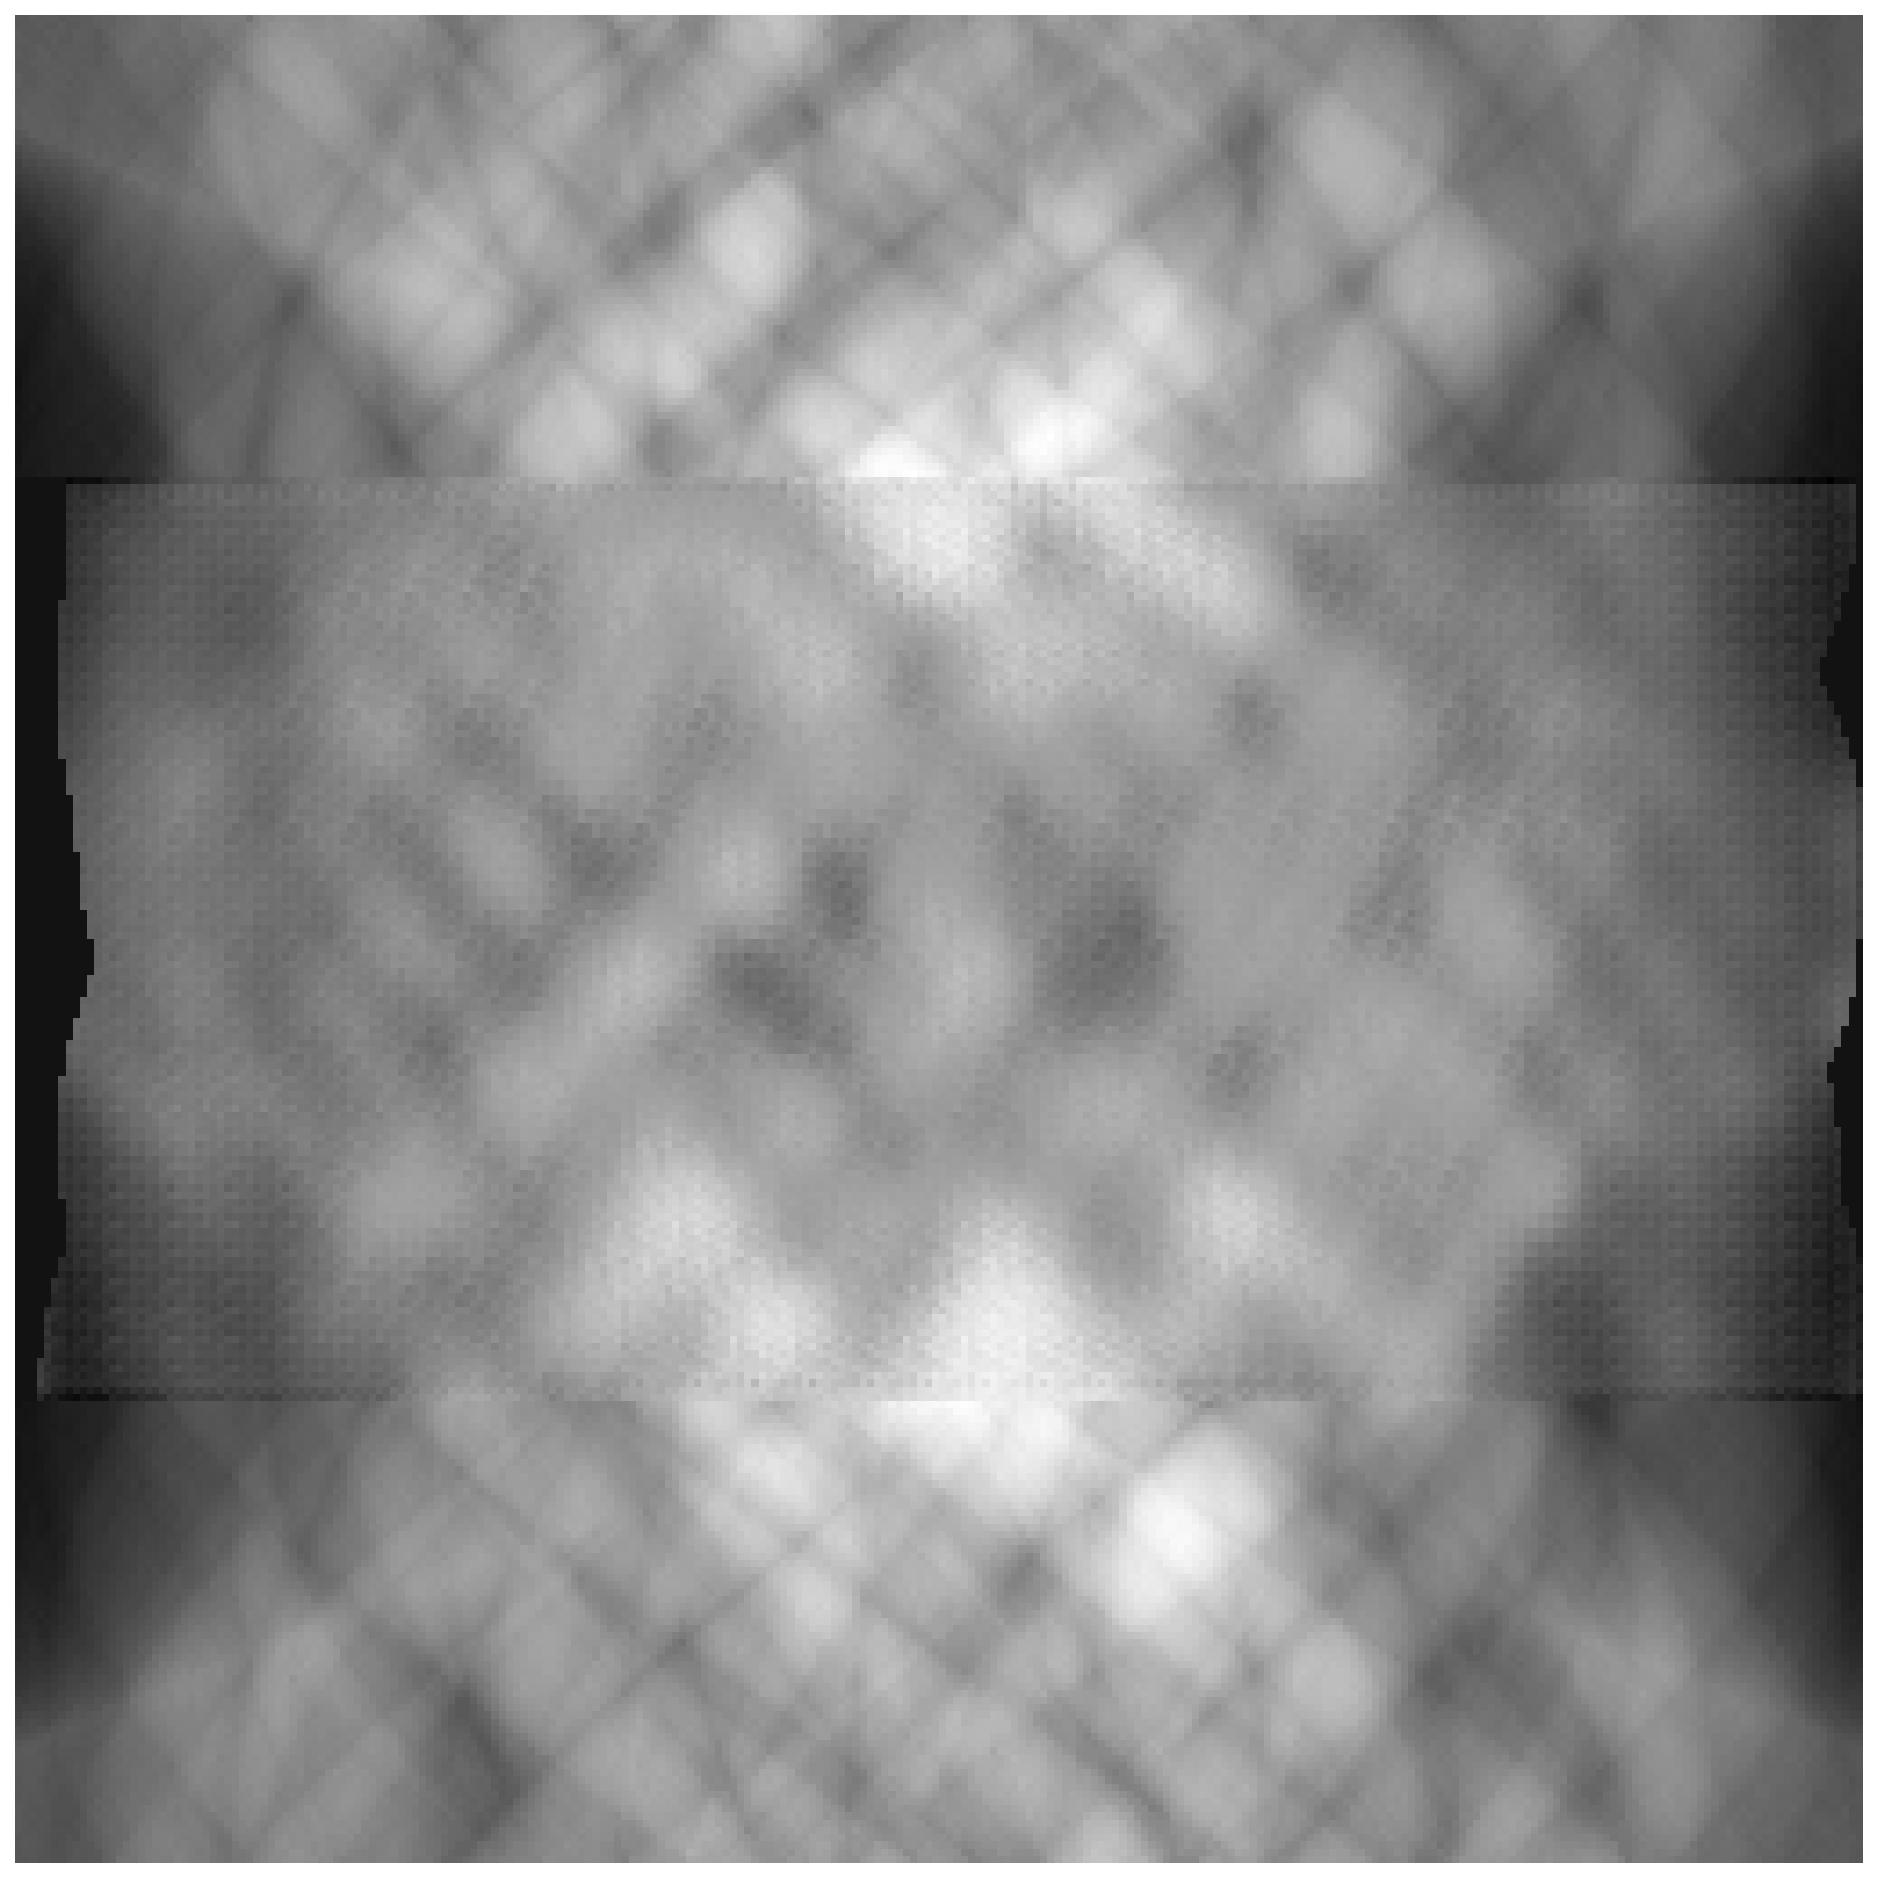
\includegraphics[width=\w\textwidth]{sinograms128_inferenceCadGan.jpg}};

\node [label={[shift={(0,-2.5)}]y}](cadSinogram) [below=5mm of scarceSinogram.south] {\includegraphics[width=\w\textwidth]{cad_sin.png}};

\draw [-latex](scarceSinogram) -- (inpainted);
\draw [-latex](cadSinogram) -| (inpainted.west);

\end{tikzpicture}
\end{frame}
\egroup


\end{document}